\documentclass{article}
\usepackage[margin=20mm]{geometry}
\usepackage{booktabs,graphicx}
\begin{document}
\title{Primary-hit spacing and MC graph fragmentation}\author{}\date{28 October 2026}\maketitle
The first 100 catalogue events per sample are used. Each actual primary
electron is ordered separately by MC time and hit ID. Consecutive stored-hit
distances are spatial chords, not G4 path lengths. The approximately 1 mm G4
step is a user-provided simulation input. No diffusion, energy threshold or
fiducial cut is applied. Coordinates and distances use Float32 mm.

Voxel centres follow the viewer convention: each coordinate is replaced by
$(\lfloor x/0.5\rfloor+0.5)0.5$ mm. Voxel-transition statistics exclude successive
hits mapped to the same cell. Revisits remain in trajectory order.

\begin{center}\small
\begin{tabular}{llrrrrr}\toprule
Sample & Positions & Pairs & Median [mm] & P99 [mm] & Max [mm] & Above 1.25 mm [\%]\\\midrule
Double beta & Original hits & 21880 & 0.930 & 0.998 & 1.000 & 0.00 \\
Double beta & Voxel centres & 19187 & 1.000 & 1.414 & 1.500 & 1.86 \\
Electrons & Original hits & 21273 & 0.970 & 0.999 & 1.003 & 0.00 \\
Electrons & Voxel centres & 19834 & 1.000 & 1.414 & 1.732 & 2.53 \\
\bottomrule\end{tabular}\end{center}
Double beta: 200 primary electrons, 0 time/hit-ID ordering disagreements, 0 equal-time pairs. 357 pairs with original separation $\leq1.05$ mm acquire a voxel separation $>1.25$ mm.

Electrons: 100 primary electrons, 0 time/hit-ID ordering disagreements, 0 equal-time pairs. 501 pairs with original separation $\leq1.05$ mm acquire a voxel separation $>1.25$ mm.

\noindent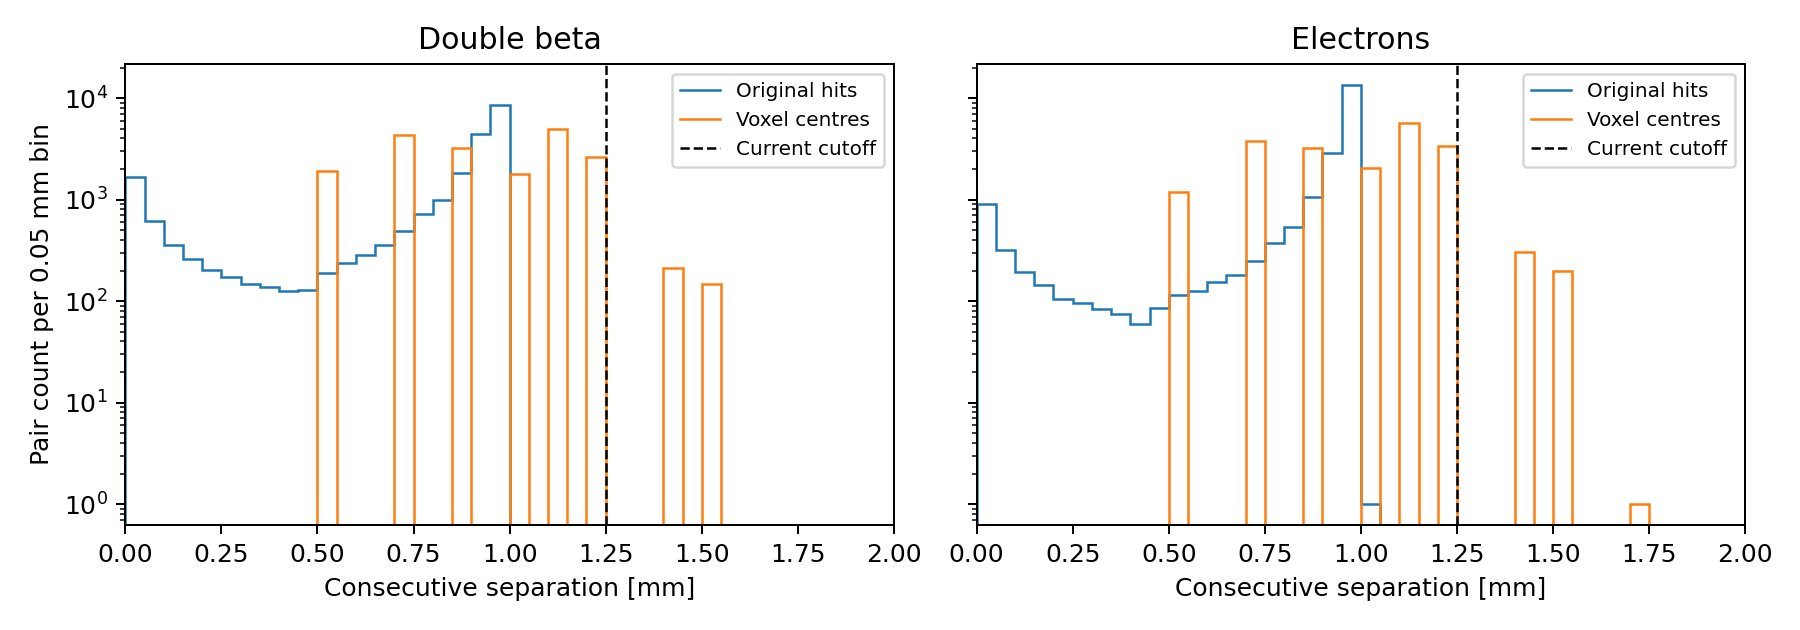
\includegraphics[width=\linewidth]{hit_spacing.png}

Every original primary-hit link in this scan passes the 1.25 mm cut.
Voxel-centre quantisation moves some of these links beyond the cut. This
directly demonstrates a source of fragmentation of a continuous primary
trajectory. All observed voxel-transition links pass a 2 mm cut. The 2 mm
radius is therefore supported for further inspection with 0.5 mm MC voxels;
this is not a measurement of background rejection or a full-sample selection
validation. Threshold removal and secondary deposits are separate effects.
Viewer settings remain unchanged.

Numerical source: \texttt{results/event\_analysis/mc\_graph\_diagnostic/hit\_spacing.h5}.
\end{document}
